\section{Nichtgleichgewichtsthermodynamik}
\subsection{Fluktuationen}
\begin{tabbing}
Reales System im Gleichgewicht zeigt kleine zeitliche Schwankungen der Observablen:
\end{tabbing}
\begin{figure}[H]
  \centering
  \begin{tikzpicture}
    \draw[->] (-0.15,0) to (10.25,0);
    \draw[->] (0,-0.15) to (0,5);
    \node at (0,5.25) {$A(t)$};
    \node at (10.5,0) {$t$};
    \draw[dashed] (0,3) to (10,3);
    \node[anchor=west] at (10.1,3) {$\langle A \rangle$};
    \draw[thick] (0,3) \foreach \x in {0.5,1,...,10} {-- (\x,3-rand)};
  \end{tikzpicture}
\end{figure}
\begin{tabbing}
Fluktuation: $\delta A(t) = A(t) - \langle A \rangle$\\
Definiere \underline{Ensemble-Mittelwert} $\langle A \rangle$ und \underline{Zeitmittelwert} $\tilde{A} = \frac{1}{T} \int\limits_0^T A(t) \dd{t} $.\\
$\langle \tilde{A} \rangle = \frac{1}{T} \int\limits_0^T \langle A(t) \rangle \dd{t} = \langle A \rangle \frac{1}{T} \int\limits_0^T \dd{t} = \rangle A \langle$\\
$\left(\Delta \tilde{A}\right)^2$\=$= \left\langle \left(\tilde{A} - \langle A \rangle\right)^2\right\rangle = \left\langle \frac{1}{T^2} \int\limits_0^T\dd{t_1}\int\limits_0^T\dd{t_2} A(t_1)A(t_2) - \langle A \rangle^2\right\rangle$\\
\>$=\frac{1}{T^2}\int\limits_0^T\dd{t_1}\int\limits_0^T \dd{t_2}\left[\langle A(t_1)A(t_2)\rangle - \langle A(t_1) \rangle\langle A(t_2) \rangle\right]$\\
Mit Definition $C(t_2 - t_1) \vcentcolon = \langle A(t_1)A(t_2)\rangle - \langle A(t_1) \rangle\langle A(t_2) \rangle$ (wegen Gleichgewicht nur von $t_2 - t_1$ abhängig)\\
\underline{Zeitkorrelationsfunktion}: $C(t) = \langle A(0)A(t)\rangle - \langle A(0) \rangle \langle A(t)\rangle$\\
\> beziehungsweise \fbox{$C(t) = \langle \delta A(0) \delta A(t)\rangle$}\\
$t = t_2 - t_1$, $t' = \frac12 (t_1 + t_2)$\\
\hspace{4em} \= \kill
$\rightarrow$\> $\left(\Delta \tilde{A}\right)^2 = \frac{2}{T} \int\limits_0^T\dd{t} (T-t) C(t)$
\end{tabbing}
\begin{figure}[H]
  \centering
  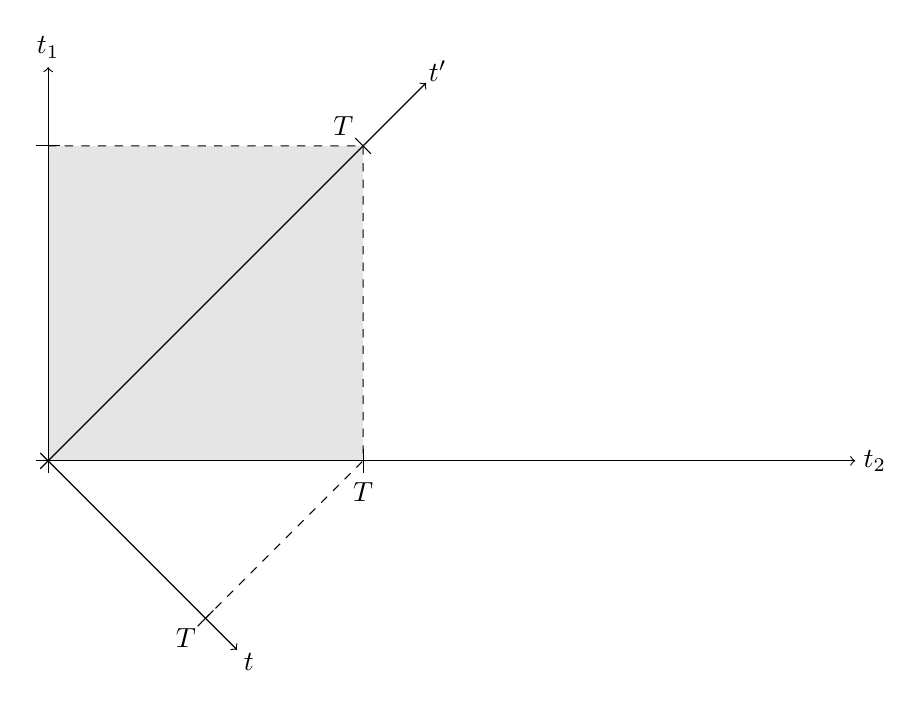
\begin{tikzpicture}
    \path[fill=white!90!black] (0,0) rectangle (4,4);
    \draw[->] (-0.15,0) to (10.25,0);
    \draw[->] (0,-0.15) to (0,5);
    \draw[->] (-0.1,-0.1) to (4.8,4.8);
    \draw[->] (-0.1,0.1) to (2.4,-2.4);
    \node at (0,5.25) {$t_1$};
    \node at (10.5,0) {$t_2$};
    \node at (4.95,4.95) {$t'$};
    \node at (2.55,-2.55) {$t$};
    \draw[dashed] (0,4) to (4,4) to (4,0) to (2,-2);
    \draw (4,-0.15) to (4,0.15);
    \draw (-0.15,4) to (0.15,4);
    \draw (4.1,3.9) to (3.9,4.1);
    \draw (1.9,-2.1) to (2.1,-1.9);
    \node at (4,-0.4) {$T$};
    \node at (3.75,4.25) {$T$};
    \node at (1.75,-2.25) {$T$};
  \end{tikzpicture}
\end{figure}
\begin{tabbing}
Falls $\int\limits_0^\infty C(t)\dd{t}$, $\int\limits_0^\infty t C(t)\dd{t}$ endlich, dann \fbox{$\left(\Delta \tilde{A}\right)^2 \sim \frac{1}{T} \to 0$} für $T \to \infty$.\\
\underline{Korrelationszeit} $\tau_C \vcentcolon = \frac{\int\limits_0^{\infty} \dd{t} t C(t)}{\int\limits_0^\infty \dd{t} C(t)}$\\
Oft: $C(t) \sim e^{-\alpha t}$ $\rightarrow$ $\tau_C = \frac{1}{\alpha}$.
\end{tabbing}


\subsection{Onsagers Regressionshypothese/ Fluktuations-Dissipationstheorem}
\begin{tabbing}
\underline{Annahme}: \= Für $t < 0$ kleine Störung $\Delta H = - f A$ des Hamiltonians\\
\> (Zum Beispiel $\Delta H  = - \vec{B}\cdot \vec{\mu}$), Gleichgewichtszustand bis $t=0$.\\
\> Für $t > 0$: $\Delta H = 0$, beobachte Zeitentwicklung $\langle A \rangle_t$.\\
$\langle A \rangle_{t = 0} = \frac{\sum\limits_j e^{-\beta(E_j + \Delta E_j)}A_j(0)}{\sum\limits_j e^{-\beta(E_j + \Delta E_j)}}$\\
$\langle A \rangle_{t} = \frac{\sum\limits_j e^{-\beta(E_j + \Delta E_j)}A_j(t)}{\sum\limits_j e^{-\beta(E_j + \Delta E_j)}}$\\
(mit $A_j(t)=$ Observable $A$ im zeitabhängigen Zustand $j$, $A_j(t) = \langle \Psi_j(t)|A|\Psi_j(t)\rangle$)\\
Näherung; $\Delta E_j$ klein\\
$\langle A \rangle_t$ \= $\approx \frac{\sum\limits_j e^{-\beta E_j}(1 - \beta \Delta E_j) A_j(t)}{\sum\limits_j e^{-\beta E_j}(1-\beta \Delta E_j)}$\\
\> $= \frac{\sum\limits_j e^{-\beta E_j}A_j(t) -\beta\sum\limits_j e^{-\beta E_j} \Delta E_j) A_j(t)}{Z\cdot\left(1 - \frac{\beta}{Z}\sum\limits_j e^{-\beta E_j}\Delta E_j\right)}$\\
\> $\approx \left(\langle A(t)\rangle - \beta \langle\Delta H A(t)\rangle \right)\cdot (1 + \beta\langle \Delta H\rangle)$\\
\> $= \langle A \rangle - \beta\langle\Delta H A(t)\rangle + \beta \langle A(t) \rangle\langle \Delta H\rangle + \mathcal{O}\left(\Delta H^2\right)$\\
$\Delta\angBra{A}_t \mDef \angBra{A}_t - \angBra{A} \approx - \beta \norBra{\angBra{\Delta H A(t)}- \angBra{A}\angBra{\Delta H}} = \beta f \norBra{\angBra{A(0)A(t)}-\angBra{A}^2}$\\
$\Delta \angBra{A}_t =$ Abweichung vom Gleichgewicht\\
\hspace{4em} \= \kill
$\rightarrow$\> \fbox{$\Delta\angBra{A}_t = \beta f \angBra{\delta A(0)\delta A(t)} = \beta f C(t)$}\\
\underline{Aussage}: Rückkehr ins Gleichgewicht (Regression, Dissipation) hängt zusammen mit spontanen Fluktuationen.
\end{tabbing}

\subsection{Mastergleichung und $H$-Theorem}
\begin{tabbing}
Betrachte System fern vom Gleichgewicht, Zustände $r$, Besetzungswahrscheinlichkeiten $P_r$.\\
Plausibel, aber nicht trivial herzuleiten:\\
$\ddv{P_r}{t} = - \sum\limits_{r'} W_{r r'} P_r + \sum\limits_{r'} W_{r' r} P_{r'} = \sum\limits_{r'} W_{r r'} \norBra{P_{r'} - P_r}$ (\underline{Mastergleichung})\\
Definiere $H(t) \mDef \sum\limits_r P_r \ln P_r$.\\
\hspace{4em} \= $\ddv{H}{t}$\= \kill
$\rightarrow$\> $\ddv{H}{t}$\>$= \sum\limits_r \norBra{\dot{P}_r\ln P_r + \dot{P}_r} = \frac{1}{2}\norBra{\sum\limits_r \dot{P}_r \ln\norBra{e P_R} + \sum\limits_{r'} \dot{P_{r'}}\ln\norBra{e P_{r'}}}$\\
\>\> $= -\frac12 \sum\limits_{r,r'} W_{r r'} \norBra{P_r - P_{r'}}\edgBra{\ln\norBra{e P_r} - \ln\norBra{e P_{r'}}}$\\
\>\> $= \frac12 \sum\limits_{r, r'} W_{r r'} \cdot P_r \cdot \norBra{1 - \frac{P_{r'}}{P_r}}\ln\frac{P_{r'}}{P_r}$\\
\hspace{4em} \= \kill
$\rightarrow$\> \fbox{$\ddv{H}{t} \leq 0$} (H-Theorem)\\
Im Gleichgewicht:  $H$ minimal und $\ddv{H}{t} = 0$.\\
Zusammenhang mit Entropie: $S = -k_B H$, maximal im Gleichgewicht\\
$\rightarrow$\> \underline{Systeme streben ins Gleichgewicht}
\end{tabbing}
